\section{Multi-resolution method }\label{numerics}

\subsection{General overview}

\begin{figure}[!htbp]
    \centering
    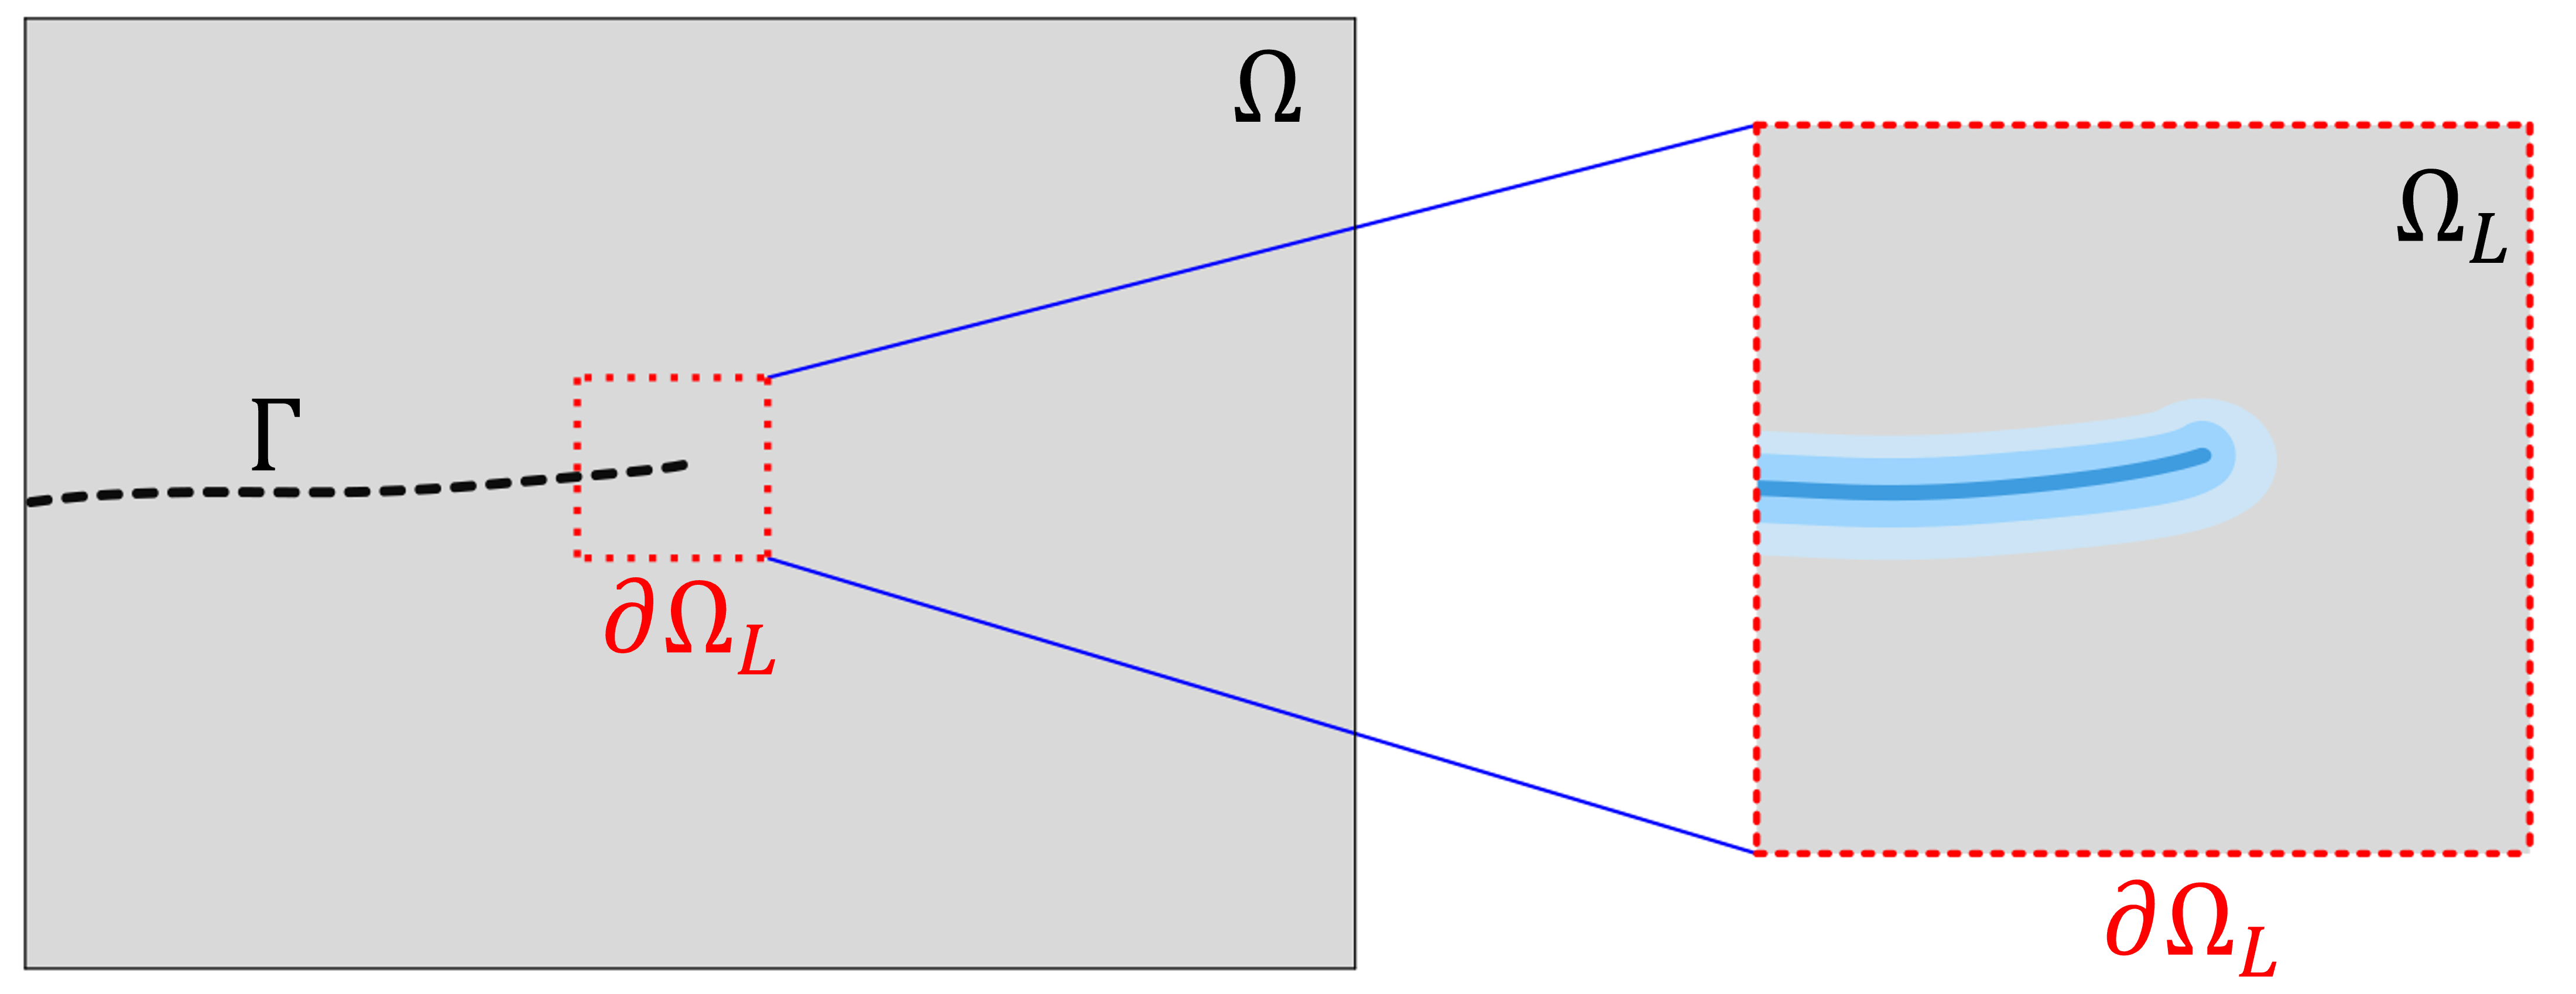
\includegraphics[width=\textwidth]{img/Section2/global_local_simple.png}
    \caption{Global domain $\Omega$ on the left and local domain $\Omega_L$ on the right. The surface corresponding to the local domain boundary $\partial\Omega_L$ is indicated within the global domain with the dashed red lines.  The local domain is magnified to highlight the phase-field representation of the global crack $\Gamma$.}
    \label{fig:section_2_figure}
\end{figure}

We propose a multi-resolution method to approximate the solution of the hydraulic fracture problem in porous media. It consists of coupling two problems between a global domain and a local subdomain, as shown in Figure~\ref{fig:section_2_figure}.   In the global domain problem, the governing equations \eqref{linear momentum balance}-\eqref{mass balance fracture} are discretized, and the crack is represented with a sharp geometry.  The crack geometry is assumed to be fixed during a solution step in the global domain, and relevant fields are calculated over the entire domain.  

By contrast, the local subdomain concerns only a portion of the entire domain, namely in the vicinity of crack tips.  It is encapsulated within the global domain as shown in Figure~\ref{fig:section_2_figure}. In the local subdomain, a discretization of the variational principle \eqref{variational formulation of phase-field} is used to simulate crack evolution.  During a solution step in the local subdomain, the pressure fields within the fracture and matrix are assumed to be fixed.  

The two problems are coupled in the following manner.  The displacement and pressure fields are extracted from a solution step in the global domain and passed to the local subproblem in different ways.  In particular, the global displacement fields are extracted along the surface $\partial\Omega_L$. These fields are then  applied as Dirichlet boundary conditions for the local subproblem.  The matrix pressure $p_m$ and pressure in the fracture $p_f$ are transfered as fields from the global domain to the local subdomain (see Section~\ref{sec:pressure_projection} for details), and assumed to be fixed for the local subproblem.   

The aforementioned operations provide everything that is needed for the local subproblem from the global domain.  Based on the imprint of the global crack geometry on the local subdomain, a regularized fracture surface is created (through an initial damage field) and then crack propagation is simulated in the local subdomain. Once an extension of the crack in a scale that can be represented in the global domain is identified, the sharp crack geometry in the global problem is updated accordingly.  

In principle, the aforementioned multi-resolution approach can be implemented using a number of different discretization methods in the global domain and the local subdomain.  In the sections that follow, we describe the particular choices used in this work as well as some important implementation details.  The method is described in a two-dimensional context, but many aspects can be readily extended to three-dimensional problems.  

\subsection{Global problem discretization}
\label{sec:global_disc}

The global problem in our multi-resolution approach encompasses the physics of fluid flow in both the fractures and the pore structure of our domain, as well as the deformation of the solid media. The set of governing equations consists of  \eqref{linear momentum balance}-\eqref{mass balance fracture}, combined with constitutive assumptions \eqref{biot law}-\eqref{poorly compressibility} and appropriate boundary conditions. 

In this work, we use the discretization method proposed by Cusini et al.\ \cite{cusini2021simulation} in the study of fluid flow in fractured porous media. 
The  domain $\Omega$ is partitioned with a  mesh $\mathcal{T}$. Then, the intersection of the fracture network $\Gamma$ with $\mathcal{T}$ defines the fracture triangulation $\mathcal{F}$. These meshes are then used to define discrete counterparts $\textbf{u}^h_G$, $p_m^h$ and $p_f^h$ of the unknown fields $\textbf{u}$, $p_m$ and $p_f$, as well as discrete approximations of equations  \eqref{linear momentum balance}, \eqref{mass balance matrix} and \eqref{mass balance fracture}.

A finite element approximation is constructed for the displacement field and employed in a standard Galerkin approximation to the global force balance \eqref{linear momentum balance}. The continuous part of the displacement field is approximated with a standard space $\mathcal{U}$  of 4-node bilinear shape functions $\{ {\boldsymbol{\eta}}_a \} $.  In the subset of elements that are ``cut" by the global crack geometry, a space $\mathcal{W}$ of discontinuous enrichment functions $\{\boldsymbol{\phi}_b\}$ is constructed using the formulation described in \cite{linder2007finite}.   

The full displacement field in the global problem is constructed using both continuous and discontinuous parts as
\begin{equation}
    \label{eq:displacement_approx}
    \textbf{u}^h_G = \underbrace{\sum_{a=1}^{n_u}u_a \boldsymbol{\eta}_a}_{\text{continuous part}} + \underbrace{\sum_{b=1}^{n_w}w_b\boldsymbol\phi_b}_{\text{discontinuous part}}, 
\end{equation}
where $\{u_a\}, \{ w_b\}$ are scalar degrees of freedom. 

The flow equations  \eqref{mass balance matrix} and \eqref{mass balance fracture} are discretized with a finite-volume method.   Piecewise-constant pressure fields are constructed for $p_m^h$ and $p_f^h$ over the matrix mesh $\mathcal{T}$ and the fracture mesh $\mathcal{F}$, respectively. Fluxes are computed using a two point flux approximation. The interaction between the flow in the fracture and matrix is effected via the embedded discrete fracture model (EDFM) \cite{lee2001hierarchical, hajibeygi2011hierarchical}. 

In terms of the temporal discretization, the parabolic nature of equations \eqref{mass balance matrix} and \eqref{mass balance fracture} gives rise to a stable time step for explicit schemes that scales with the cube of the mesh spacing \cite{adachi2007computer, lecampion2018numerical}. This upper bound is prohibitively small in most cases. Therefore, an implicit backward Euler method is used throughout. This gives rise to a fully-coupled system of nonlinear equations, whose solution is obtained with a Newton method, in a monolithic fashion. 

One limitation of the construction \eqref{eq:displacement_approx} is that the discontinuous enrichment functions are not capable of representing a crack tip that terminates inside of an element.  As such, any new extension of the crack geometry has to traverse from one side of a new element to another. The implementation of the fracture flow solver requires all cells to have non-zero volumes.  Accordingly, new fracture cells are assigned a  small aperture value ($w_0$). The total discrete aperture of the cell is thus given by $w_h = w_n + w_0$, where $w_n$ is the mechanical aperture that is consistent with the jump provided by the displacement field.  The minimum opening $w_0$ has been interpreted as a representation of the roughness of the fracture surfaces, providing a pathway for fluid flow even when the cracks are mechanically closed.  See, for example \cite{cusini2021simulation}.

\subsection{Local problem initialization} 

\subsubsection{Construction of subdomain, submesh and damage-fixed nodes}\label{subdomain_construction}

A local subdomain of size $L\times L$ is constructed by simply centering it on a global crack tip.  The size $L$ is selected to be an even integer multiplier of the global mesh spacing, leading to a square bounding box that conforms to the background mesh.  This choice is adopted for convenience in this work, although other constructions are possible, such as in  \cite{giovanardi2017hybrid}.

To obtain the submesh $\mathcal{T}_L$, we start by considering the restriction of the global triangulation $\mathcal{T}$ to the subdomain $\Omega_L$.  The mesh for the local subdomain is constructed by uniformly refining the set of elements in this restriction. This facilitates the transfer of nodal data from the global to the local problem.  The mesh size $h_{local}$ in the local subdomain is chosen to be sufficiently small to resolve the damage band, of size $\mathcal{O}(\ell)$. In this work, we use  $\ell / h_{local} \approx 4$.

\begin{figure}[h]
    \centering
    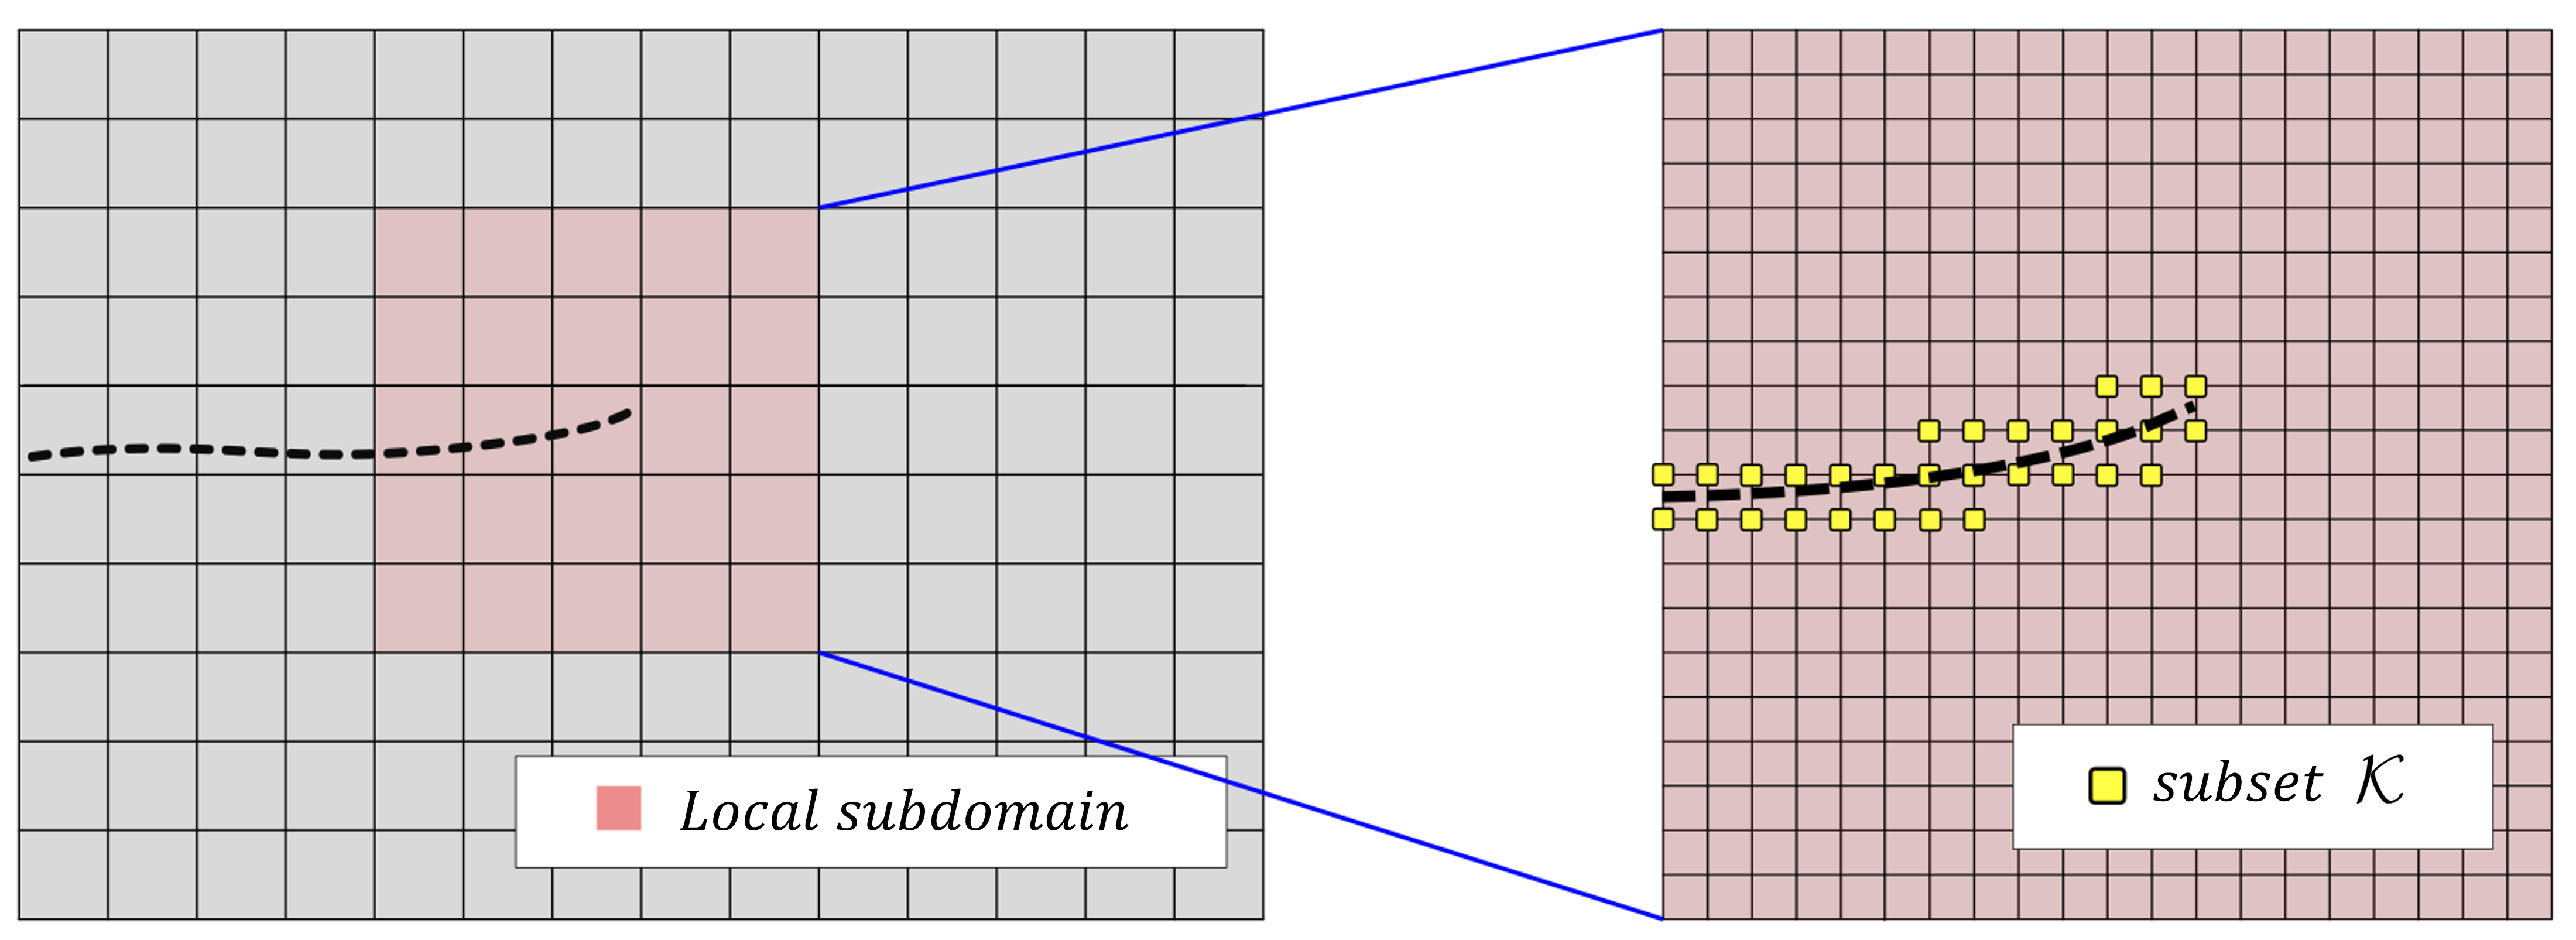
\includegraphics[width=\textwidth]{img/Section2/subset_kappa.png}
    \caption{Global domain $\Omega$ on the left and local domain $\Omega_L$ on the right. The nodes in the subset $\mathcal{K}$, where $d$ is set to $1$ are colored in yellow.}
    \label{fig:subset_kappa}
\end{figure} 

The crack is represented by prescribing $d = 1$ in a set $\mathcal{K} \in \mathcal{T}_L$ of nodes in the local subdomain, as shown in Figure \ref{fig:subset_kappa}. This set is constructed in two steps. First, all elements of $\mathcal{T}_L$ which are intersected by the global fracture triangulation $\mathcal{F}$ are identified.  Then, $\mathcal{K}$ is defined to be the set of all nodes that belong to any of these intersected elements.

\subsubsection{Transfer of global pressures to local mesh}
\label{sec:pressure_projection}

Due to the different levels of resolution between the global and local problems, we find it advantageous to transfer the pressure fields in a particular manner.  We note that in the global problem, the fracture pressures $p_f^h$ are available at the cell centers of 1D finite volumes, and the matrix pressures $p_m^h$ are available at the cell centers of 2D finite volumes.  These fields are transferred to quadrature points in the finite element mesh for the local subproblem using the transfer operators 
$\Pi^{\Omega_L}_f$ and $\Pi^{\Omega_L}_m$.

\begin{figure}[!htbp]
    \centering
    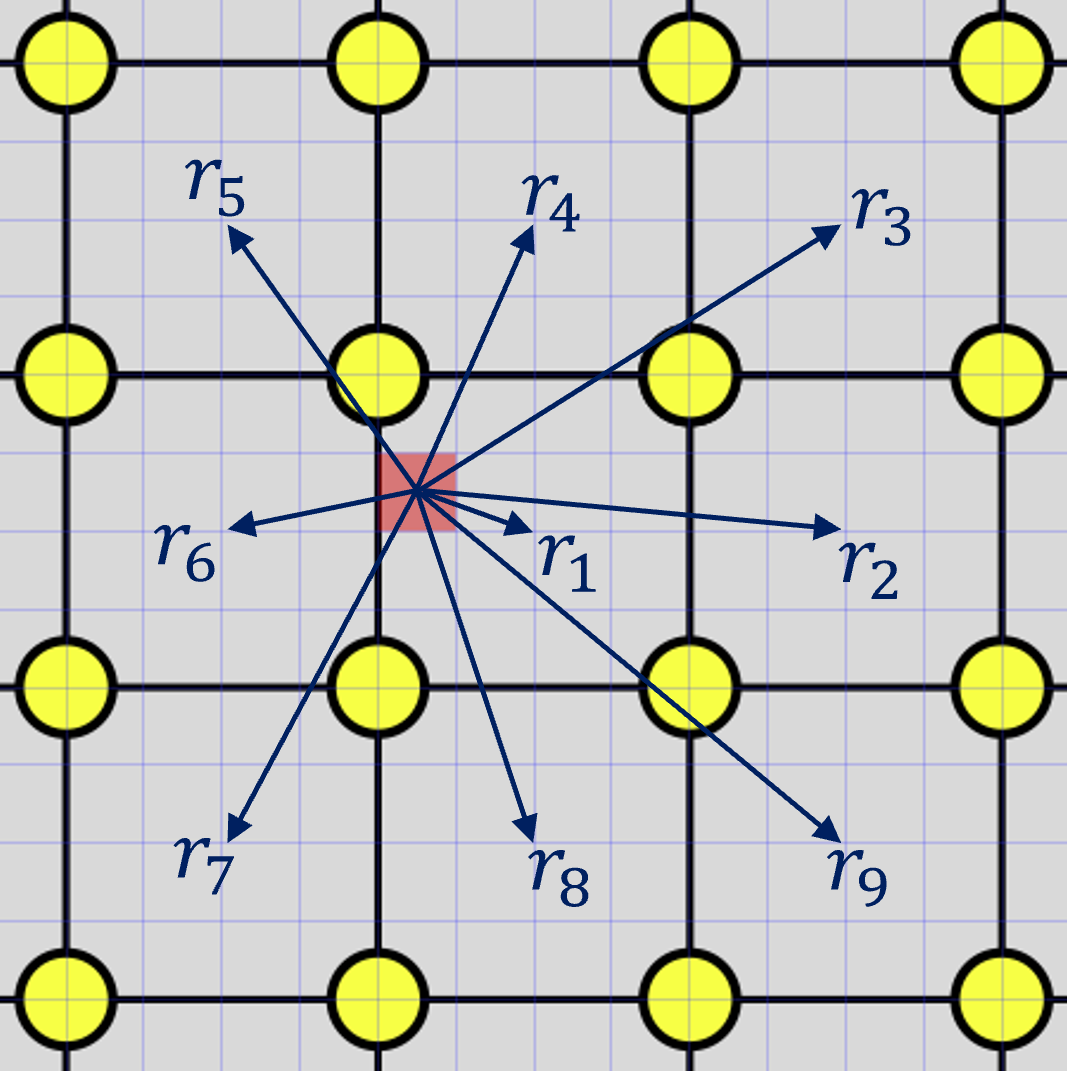
\includegraphics[width=6cm]{img/Section2/pressure_interpolation_blue_small.png}
    \caption{Illustration of global cells (in gray) in the neighborhood of a local element, indicated in pink. The matrix pressure at a quadrature point in the local element is calculated using an average of global pressures from neighboring cells $\{ i \}$, with weights corresponding to the distances $r_i$ between the quadrature point and the cell center.}
    \label{fig:pressure_interpolation}
\end{figure}

The operator $\Pi^{\Omega_L}_f$ that transfers the fracture pressure is straightforward, and inspired by a similar operation described in Santillán et al.\ \cite{santillan2018phase}. Given any point $ {\bf{x}} \in \Omega_L$, and a global fracture pressure field $p_f^h$, $\Pi^{\Omega_L}_fp_f^h({\bf{x}})$ is obtained by finding the closest cell of $\mathcal{F}$ to $x$ and taking the value of $p_f^h$ at this cell. More precisely,

\begin{equation}
    \Pi^{\Omega_L}_f p_f^h({\bf{x}}) = p_f^h(\underset{c \in \mathcal{F}}{\text{arg min }}\text{dist}(c,{\bf{x}} )).
\end{equation}

For the operator $\Pi^{\Omega_L}_m$ that transfers the matrix pressure field, we use an averaging procedure.  This has the effect of smoothing the matrix pressure field at the resolution of the local mesh.  At a quadrature point ${\bf{x}}_Q \in \Omega_L$, the matrix pressure in the local domain is obtained from a weighted average of the pressures in the global cells that surround the point.  Specifically, 
\begin{equation}
    \Pi^{\Omega_L}_m p_m^h({\bf{x}}_Q) = \dfrac{\sum_{i=1}^s r^{-1}_ip_m^h(c_i)}{\sum_{i=1}^s r^{-1}_i},
\end{equation}
where $r_i$ denotes the distance between the quadrature point location and the center of global cell $i$, as indicated in Figure~\ref{fig:pressure_interpolation}.  In the sum, all cells that neighbor the global cell containing quadrature point ${\bf{x}}_Q$ are used.  In the particular case when a quadrature point happens to reside in the center of the local element and $r_1 = 0$, the above sum is replaced with   
$ \Pi^{\Omega_L}_mp_m^h({\bf{x}}_Q) = p^h_m (c_1)$.

\subsection{Local problem discretization}

With the local subdomain properly identified and initialized, we now describe the additional steps to discretize the displacement and damage fields in the local subdomain and solve for their approximations.
The governing equations for the macro-force balance \eqref{basic u problem} and the damage evolution \eqref{damage equation ch3} are both treated with the finite element method.  The damage and displacement fields are both approximated using four-node bilinear quadrilateral elements. 

Let $\Omega_L$ denote the local domain. From the finite-element approximation $\textbf{u}_G^h$ computed in the global problem, we extract $\textbf{u}^h_G|_{\partial\Omega_L}$ and use it to constrain the displacements on the boundary of the subproblem \footnote{In the multi-resolution method of Muixi et al.\ \cite{muixi2021combined},  the displacement boundary conditions near the crack base were released. We did not find this to be necessary in our approach.}.  As such, the trial space $\boldsymbol{\mathcal{U}}^h$ is given by
\begin{equation}\label{disp subspace}
    \boldsymbol{\mathcal{U}}^h = \{ \textbf{u}_L^h \in H^1(\Omega_L)^n \mid \textbf{u}_L^h = \textbf{u}^h_G \text{ on } \partial\Omega_L \}.
\end{equation}

The function space $\mathcal{D}^h$ of admissible damage fields is given by 
\begin{equation}\label{damage subspace}
    \mathcal{D}^h = \{ d^h \in H^1(\Omega_L) \mid d^h = 1 \text{ on } \mathcal{K} \},
\end{equation}
where $\mathcal{K}$ denotes the set of damage-fixed nodes that correspond to the global crack at the beginning of the load step, as described in subsection~\ref{subdomain_construction}. 

The test spaces are given by $\boldsymbol{\mathcal{W}}^h = H_0^1(\Omega_L)^n$ for the displacements and $\mathcal{C}^h = \{ c^h \in H^1(\Omega_L) \mid c^h = 0 \text{ on } \mathcal{K} \}$ for the damage field. The Galerkin approximation to the problem on the local subdomain is then:
\medskip

\begin{mdframed}[
    frametitle={The spatially discrete form},
    frametitlebackgroundcolor=gray!20,
    backgroundcolor=gray!5,
    linewidth=0pt,
    nobreak=true
  ]
  Find $\textbf{u}_L^h \in \boldsymbol{\mathcal{U}}^h$ and $d^h \in \mathcal{D}^h$, such that $\forall \textbf{w}^h \in \boldsymbol{\mathcal{W}}^h$ and $\forall c^h \in \mathcal{C}^h$,
 
 \begin{align}
  \left( \nabla \textbf{w}^h, \boldsymbol\sigma_L^h \right) - \left( \textbf{w}^h, \Pi^{\Omega_L}_f p_f^h \nabla d^h \right) - \left( \textbf{w}^h, \textbf{b} \right) - \left< \textbf{w}^h, \textbf{t} \right>_{\partial_t\Omega} &= 0, \label{eq: semidiscrete momentum balance ch3}   \\
  \begin{split}
    \frac{2G_c^h\ell}{c_0}\left( \nabla c^h, \nabla d^h \right) + \frac{G_c^h}{c_0\ell}\left( c^h, \zeta'(d^h) \right) + \left( c^h, 2(d^h-1)W(\boldsymbol{\epsilon^+}(\textbf{u}_L^h),0) \right) \\
    + \left( c^h, \alpha \Pi^{\Omega_L}_m p_m^h\nabla \cdot \textbf{u}_L^h \right) + \left( \nabla c^h, \Pi^{\Omega_L}_f p_f^h\textbf{u}_L^h \right)  &= 0, \label{eq: semidiscrete damage evolution}    
  \end{split} 
\end{align}

\end{mdframed}
where we have used $(\cdot,\cdot)$ to denote the standard inner product in the $L^2(\Omega)$ space, and $\left< \cdot, \cdot \right>$ to denote its restriction on the boundary.   In the above,  $\boldsymbol\sigma^h_L$ denotes the discrete stress, given by 
\begin{equation}
    \boldsymbol\sigma^h_L = \left( (1-d^h)^2\ \mathbb{C}:\boldsymbol\epsilon(\textbf{u}_L^h) -(1-d^h)\alpha p_m^h \mathbb{I}\right).
\end{equation}

We employ an alternating minimization scheme to solve the coupled system of equations \eqref{eq: semidiscrete momentum balance ch3}-\eqref{eq: semidiscrete damage evolution}. Convergence is measured with respect to the $L_2$-norms of the change in the damage $d^h$ and  displacement fields $\textbf{u}_L^h$, using a relative tolerance of $10^{-4}$. With this approach, each of the equations becomes linear with respect to its primary variable, simplifying the solution process.

We note that \eqref{eq: semidiscrete damage evolution} does not explicitly include the irreversibility constraint  \eqref{eq:ddot-strong}. Within the multi-resolution scheme, the Dirichlet condition $d^h=1$ on the crack set $\mathcal{K}$ is sufficient to prevent the healing of the fracture surface relative to the initial global crack.  It does not, however, enforce irreversibility of the damage throughout the local subdomain, and it is possible that some crack healing could occur if regions are loaded and unloaded during a single time step.  
We did not find this to occur for the problems studied in this work, but it is possible that this could arise in more complex cases and the use of a more robust means of enforcing the constraint on the damage would be needed.  Options include, for example, the active set solver described in \cite{hu2020frictionless}.   

In terms of the local dissipation function $\zeta(d)$, in this work we use $\zeta(d) = d$ which corresponds to the AT-1 phase-field model of fracture.  This is selected due to the fact that it gives rise to a compactly supported damage field and a fully elastic stage prior to damage initiation \cite{pham2011gradient}.
When using the AT-1 model, it is necessary to explicitly enforce the constraint $d^h \ge 0$, as in some cases, this formulation can lead to negative damage values. In this work, this is effected  by invoking a lower threshold on the active part of the strain energy $W(\boldsymbol{\epsilon^+}(\textbf{u}_L^h),0) = 3G_c/8\ell$, as in \cite{miehe2016phase}. 

Finally, we note that phase-field models of fracture tend to give rise to a mesh and regularization length dependent critical fracture energy that is larger than $G_c$ \cite{bourdin2008variational}.  To account for this, we use a discrete value of $G_c^h$ that is obtained as a function of the local mesh spacing and regularization length, as
    \begin{equation}
        G_c^h = G_c \left( 1 + \dfrac{ h_{local} }{c_0\ell} \right)^{-1},
    \end{equation}
such that the effective critical fracture energy is very close to that of the material.  

\subsection{Crack propagation: translating local damage updates into global crack extensions}\label{propagation_step}


A key step of the algorithm concerns how changes to the damage in the local subdomain are translated into updates to the crack geometry in the global domain.  We provide details of our algorithm for this procedure here.  The scheme is presented in the context of a single crack tip that is propagating through the global domain. Although we do not consider much more complex cases in this work, such as changes in crack topology (due to crack branching or merging), we note that such problems have been examined in other works employing hybrid phase-field approaches.  This includes the recent work of Muixi et al.~\cite{muixi2021combined}, albeit in a purely mechanical context.

At each step in the solution algorithm, in the global problem, we keep track of two geometric entities, namely the global crack tip and the global tip element (Figure \ref{fig:all_tips}a). The global crack tip is defined by the interior endpoint of the crack.  The global tip element is the element that contains the tip on one of its sides, but is not yet ``cut" by the crack.  In essence, it is the global element just ahead of the propagating crack tip.   In the local subproblem, we identify a local version of the crack tip that is obtained from the discrete damage field $d^h$ (Figure \ref{fig:all_tips}b and \ref{fig:all_tips}c).  
The algorithm to extend the global crack geometry depends on the relative location of the global crack tip, global tip element, and local crack tip, as described below.

\begin{figure}[!h]
\centering
\begin{subfigure}{.33\textwidth}
  \centering
  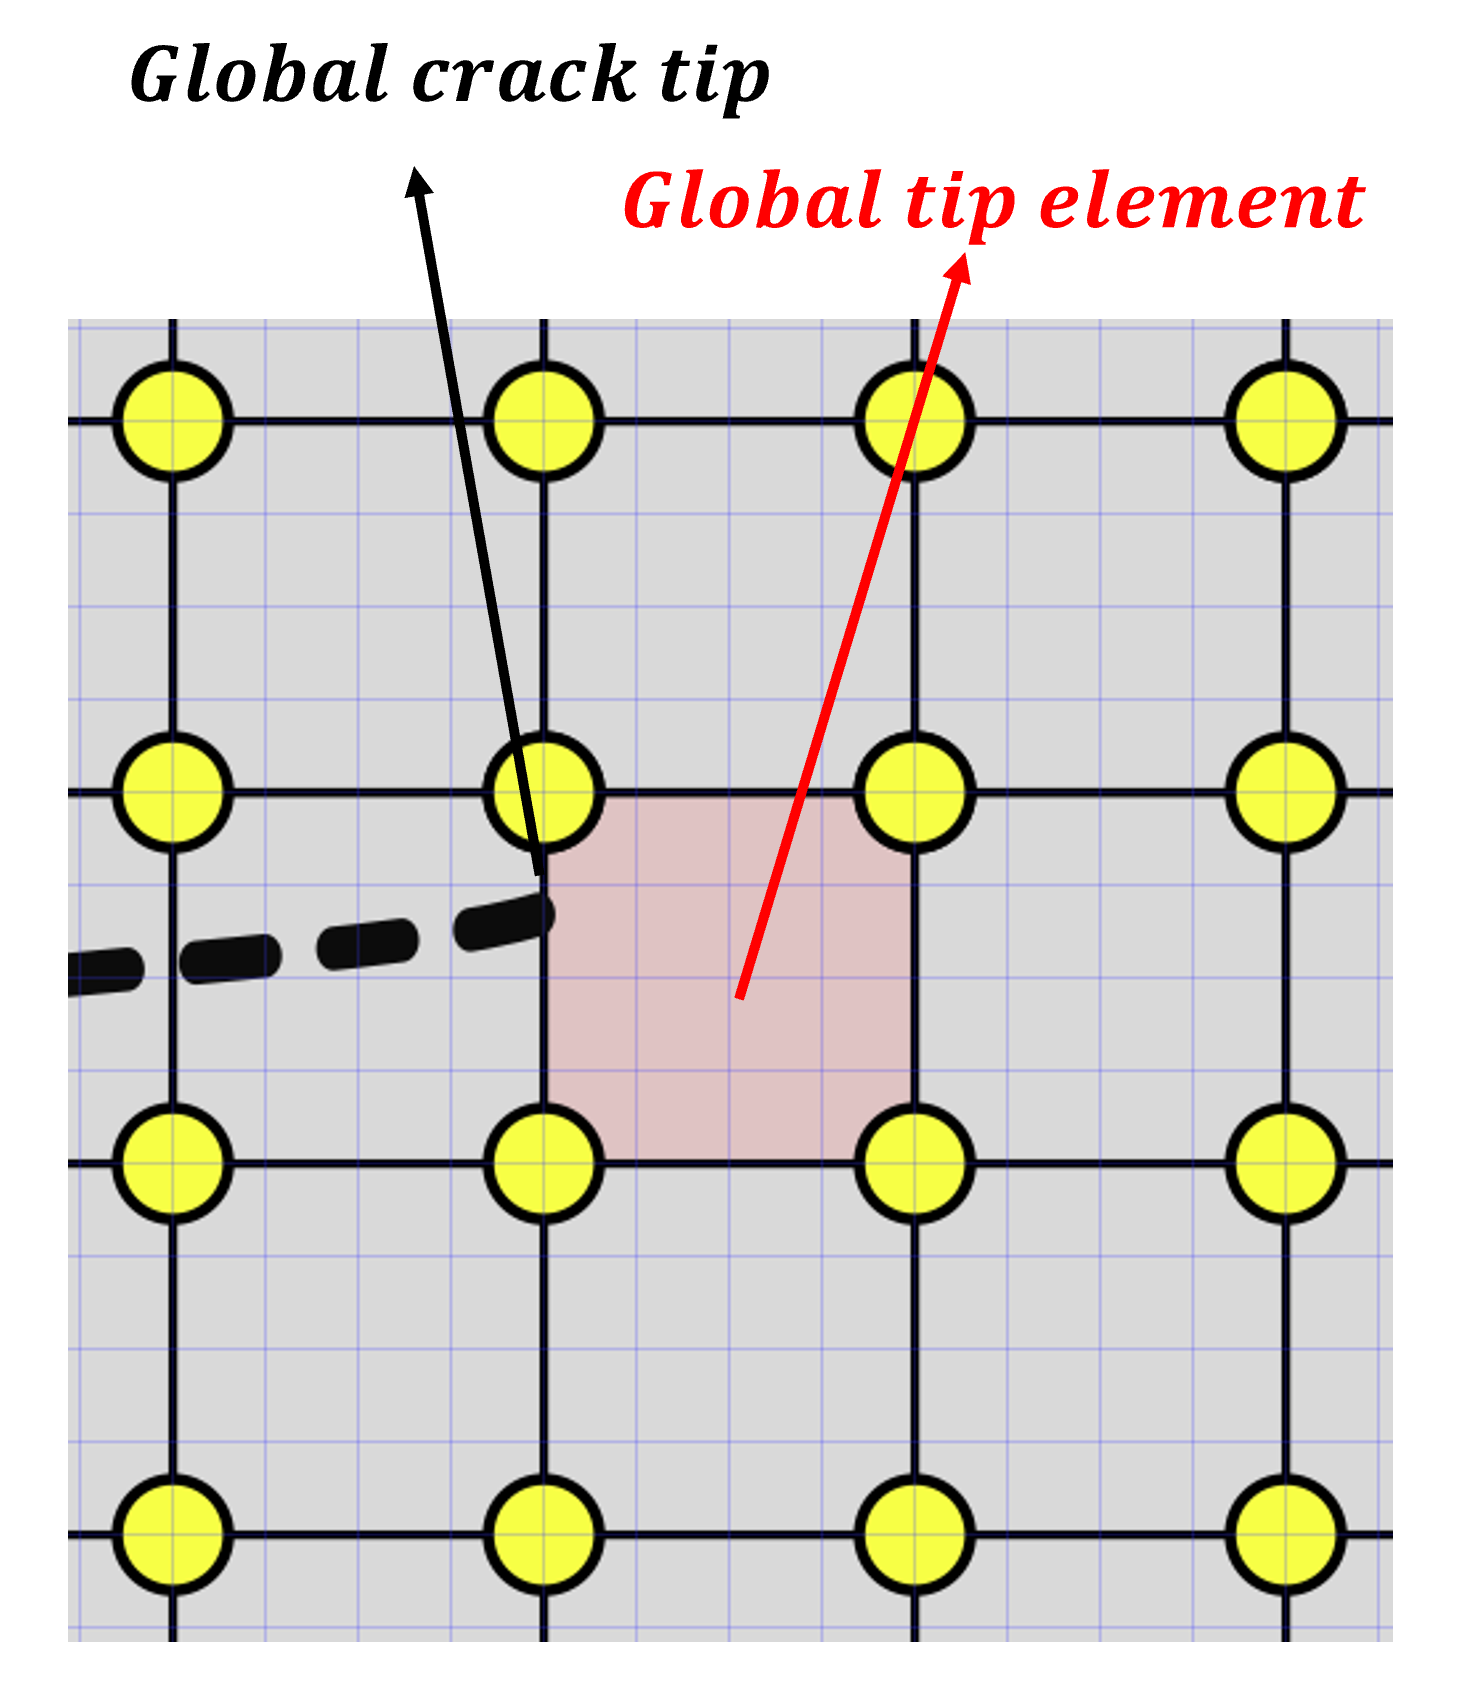
\includegraphics[width=\linewidth]{img/Section2/propagation_items_1.png}
  \caption{}
  \label{fig:prop_items}
\end{subfigure}%
\begin{subfigure}{.33\textwidth}
  \centering
  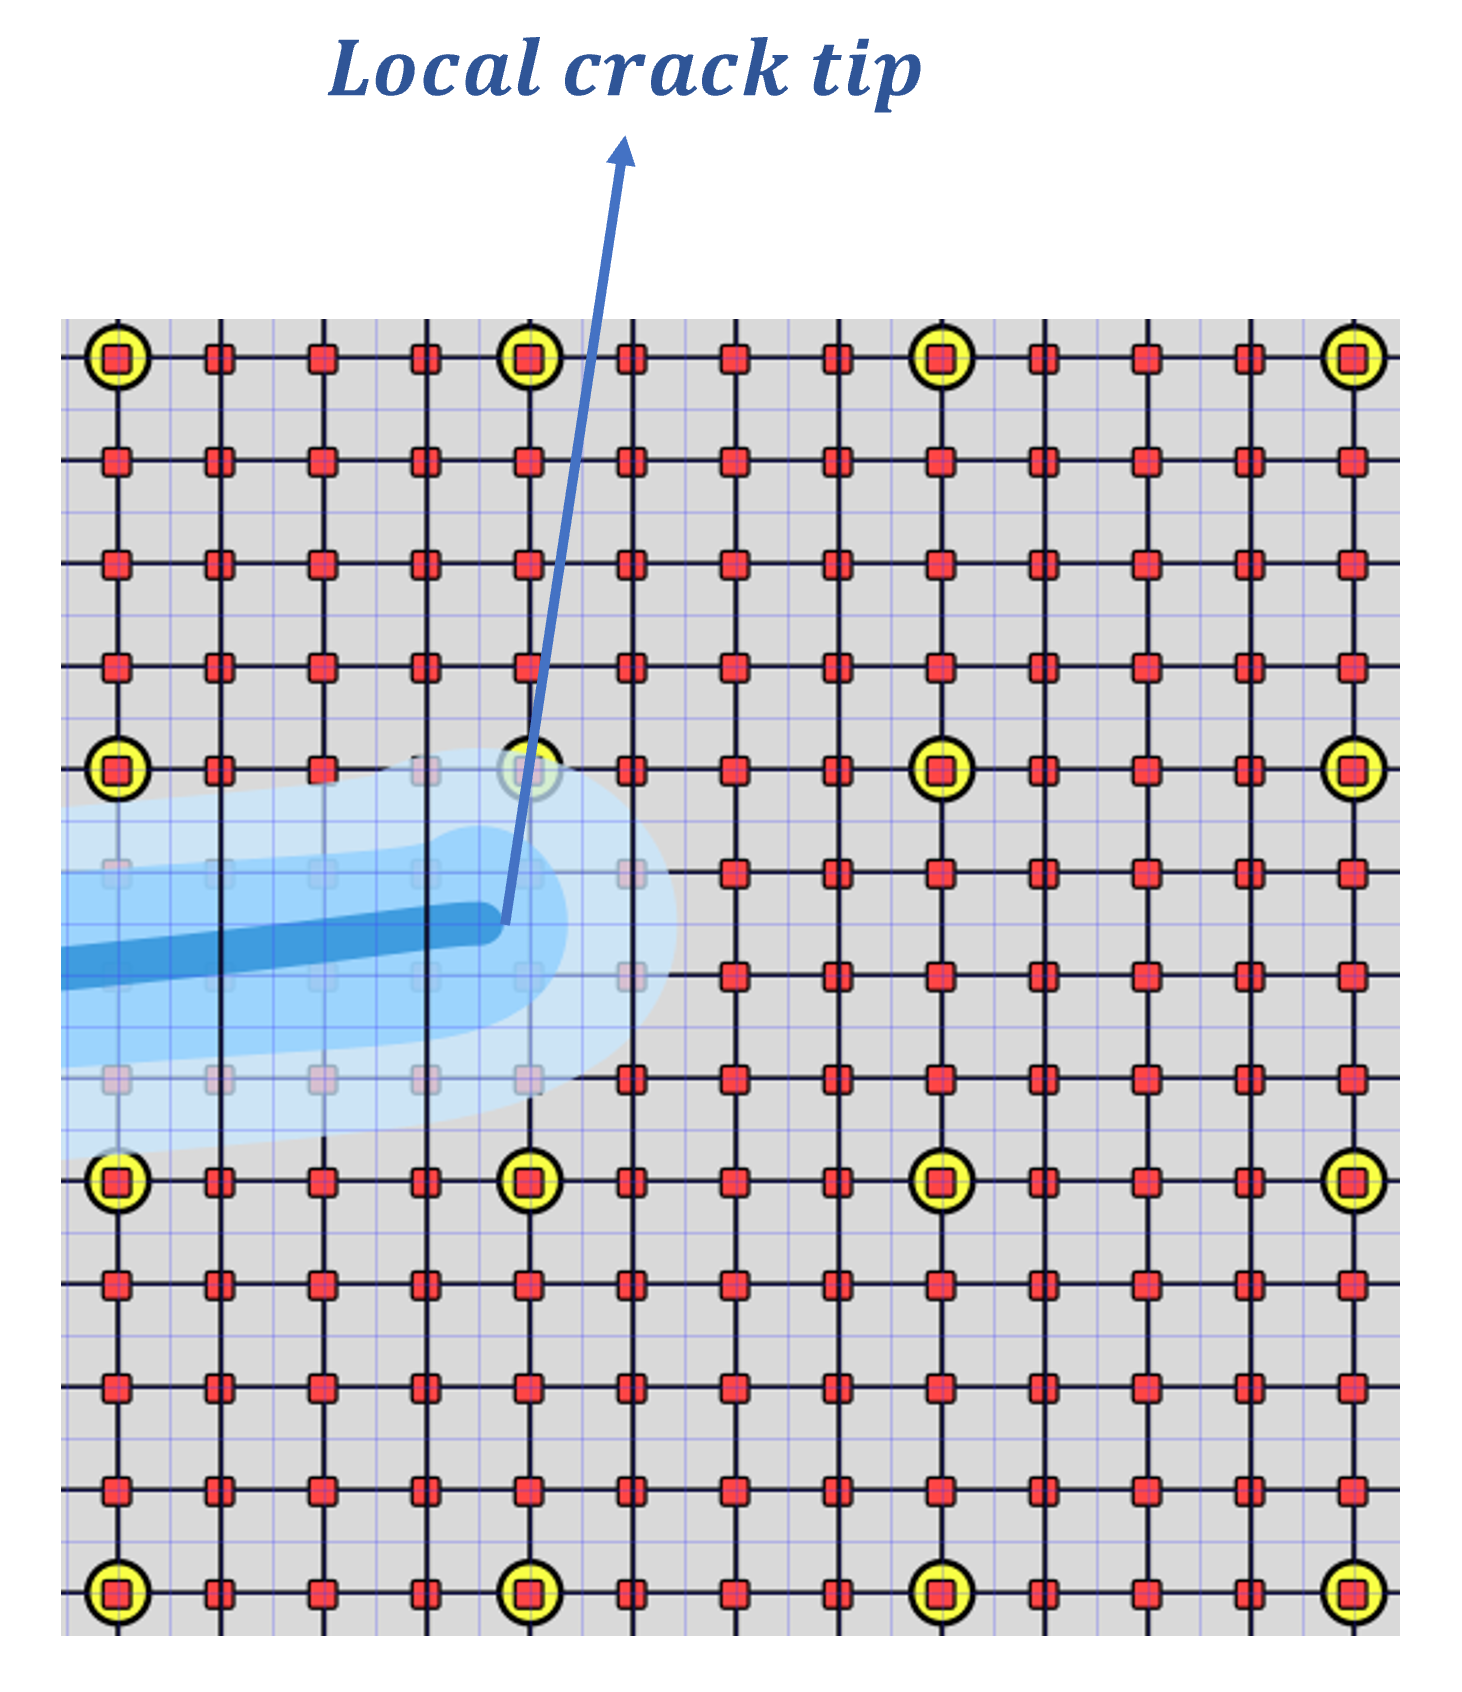
\includegraphics[width=\linewidth]{img/Section2/propagation_items_2.png}
  \caption{}
  \label{fig:prop_items2}
\end{subfigure}
\begin{subfigure}{.33\textwidth}
  \centering
  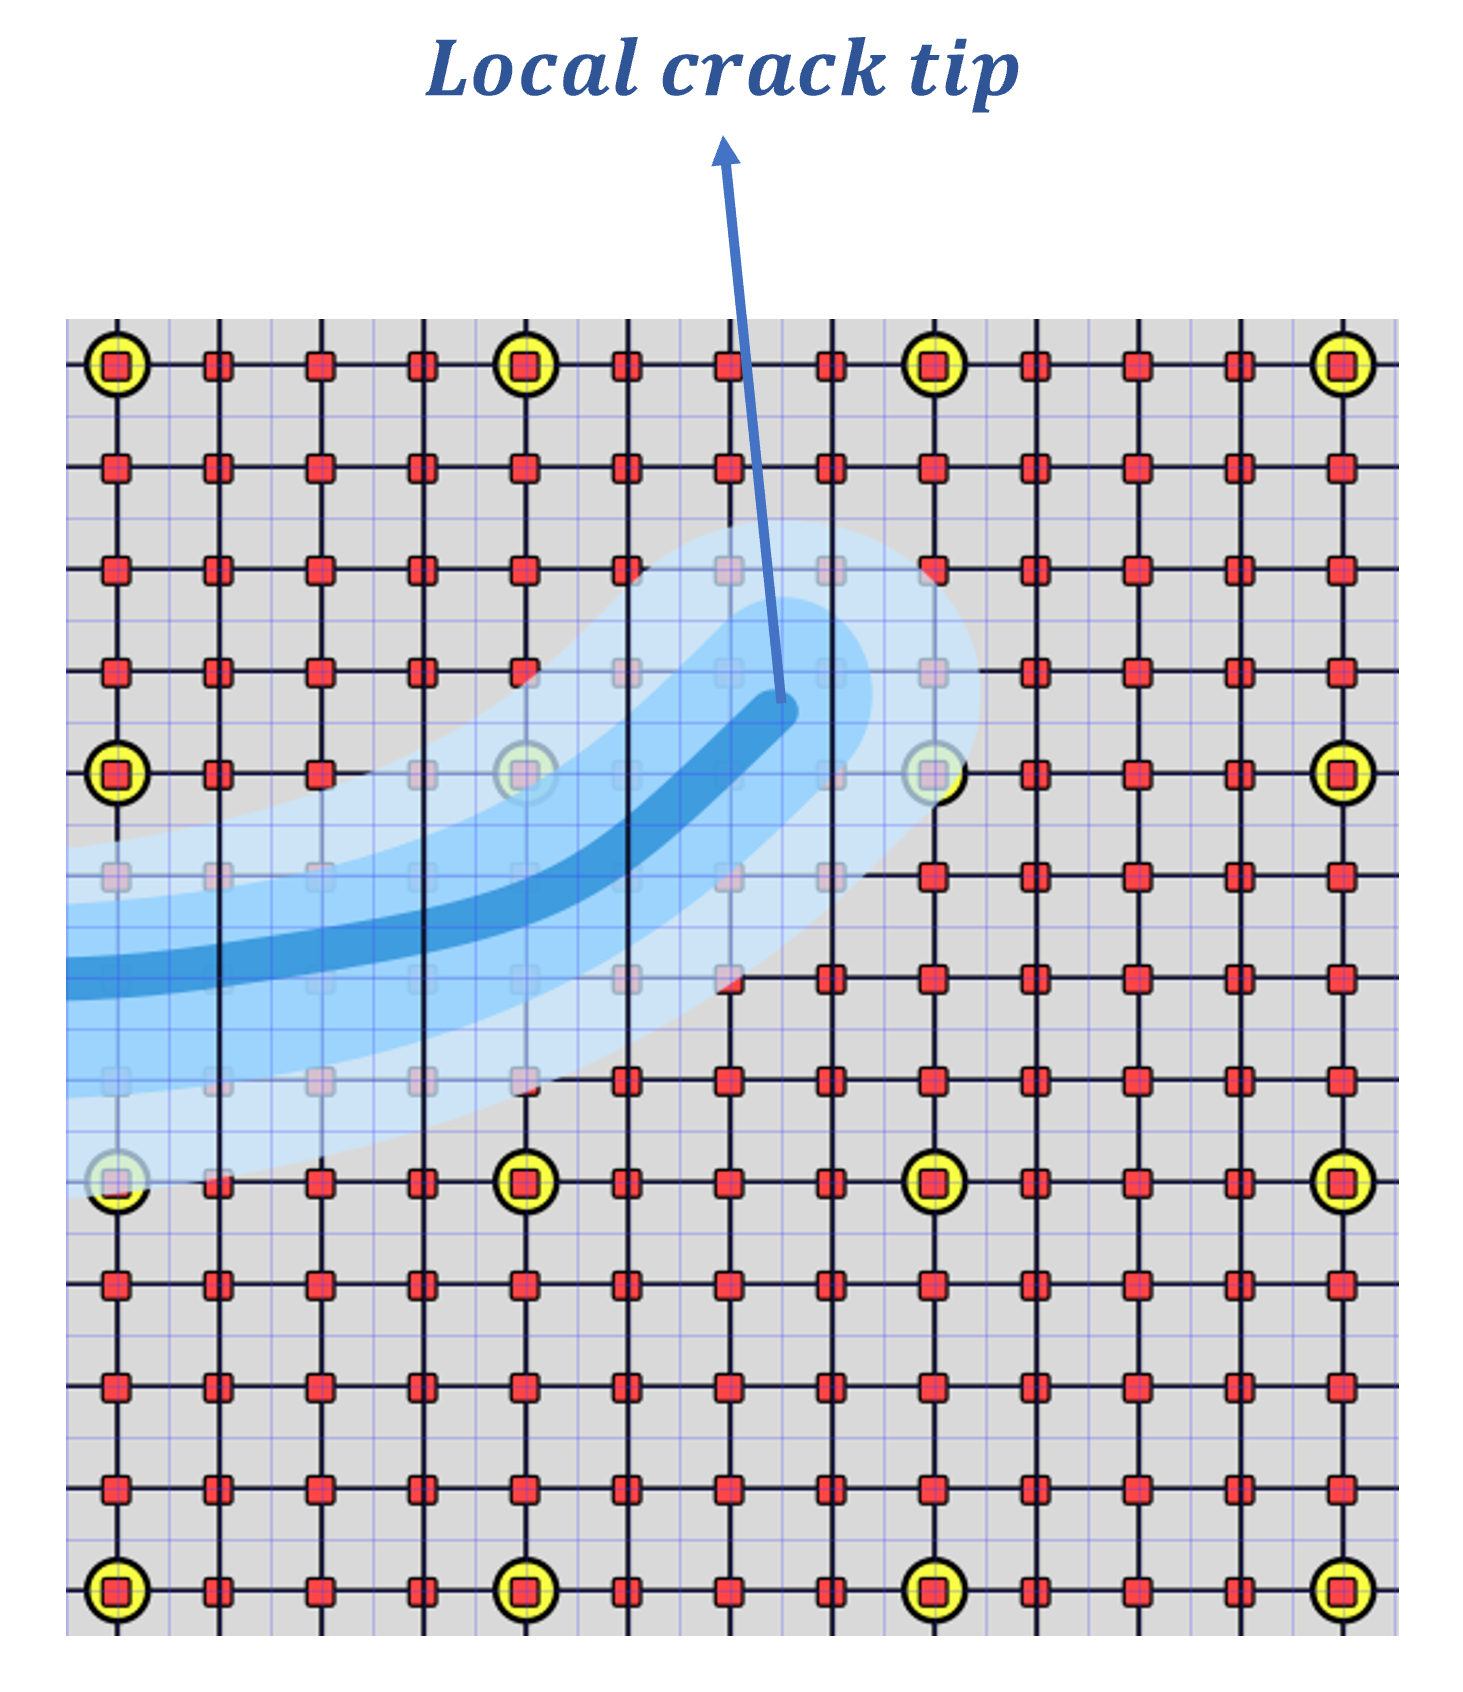
\includegraphics[width=\linewidth]{img/Section2/propagation_items_3.png}
  \caption{}
  \label{fig:prop_items3}
\end{subfigure}
\caption{(a): Illustration of the global crack tip and global tip element. (b) Case when the local tip falls inside the tip element. (c) Case when the local tip falls outside the tip element.}
  \label{fig:all_tips}
\end{figure}

The enrichment strategy described in Section~\ref{sec:global_disc} requires global elements that are completely cut by the crack geometry.  As such, any extension of the crack geometry at the global scale must correspond to the global tip element being fractured.  Accordingly, global crack propagation is triggered whenever the local tip falls outside the tip element. In this case, the new global tip is identified by connecting the current global tip and the local tip. Since the local tip is outside the tip element, a new segment will intersect the perimeter of the tip element exactly once (neglecting the obvious intersection at the current global tip). This process is illustrated in Figure \ref{fig:tip_progression}. Any crack advance beyond this new tip location is neglected at this point, and the algorithm returns to a new global solve with an updated crack geometry.  

\begin{figure}
\centering
\begin{subfigure}{.331\textwidth}
  \centering
  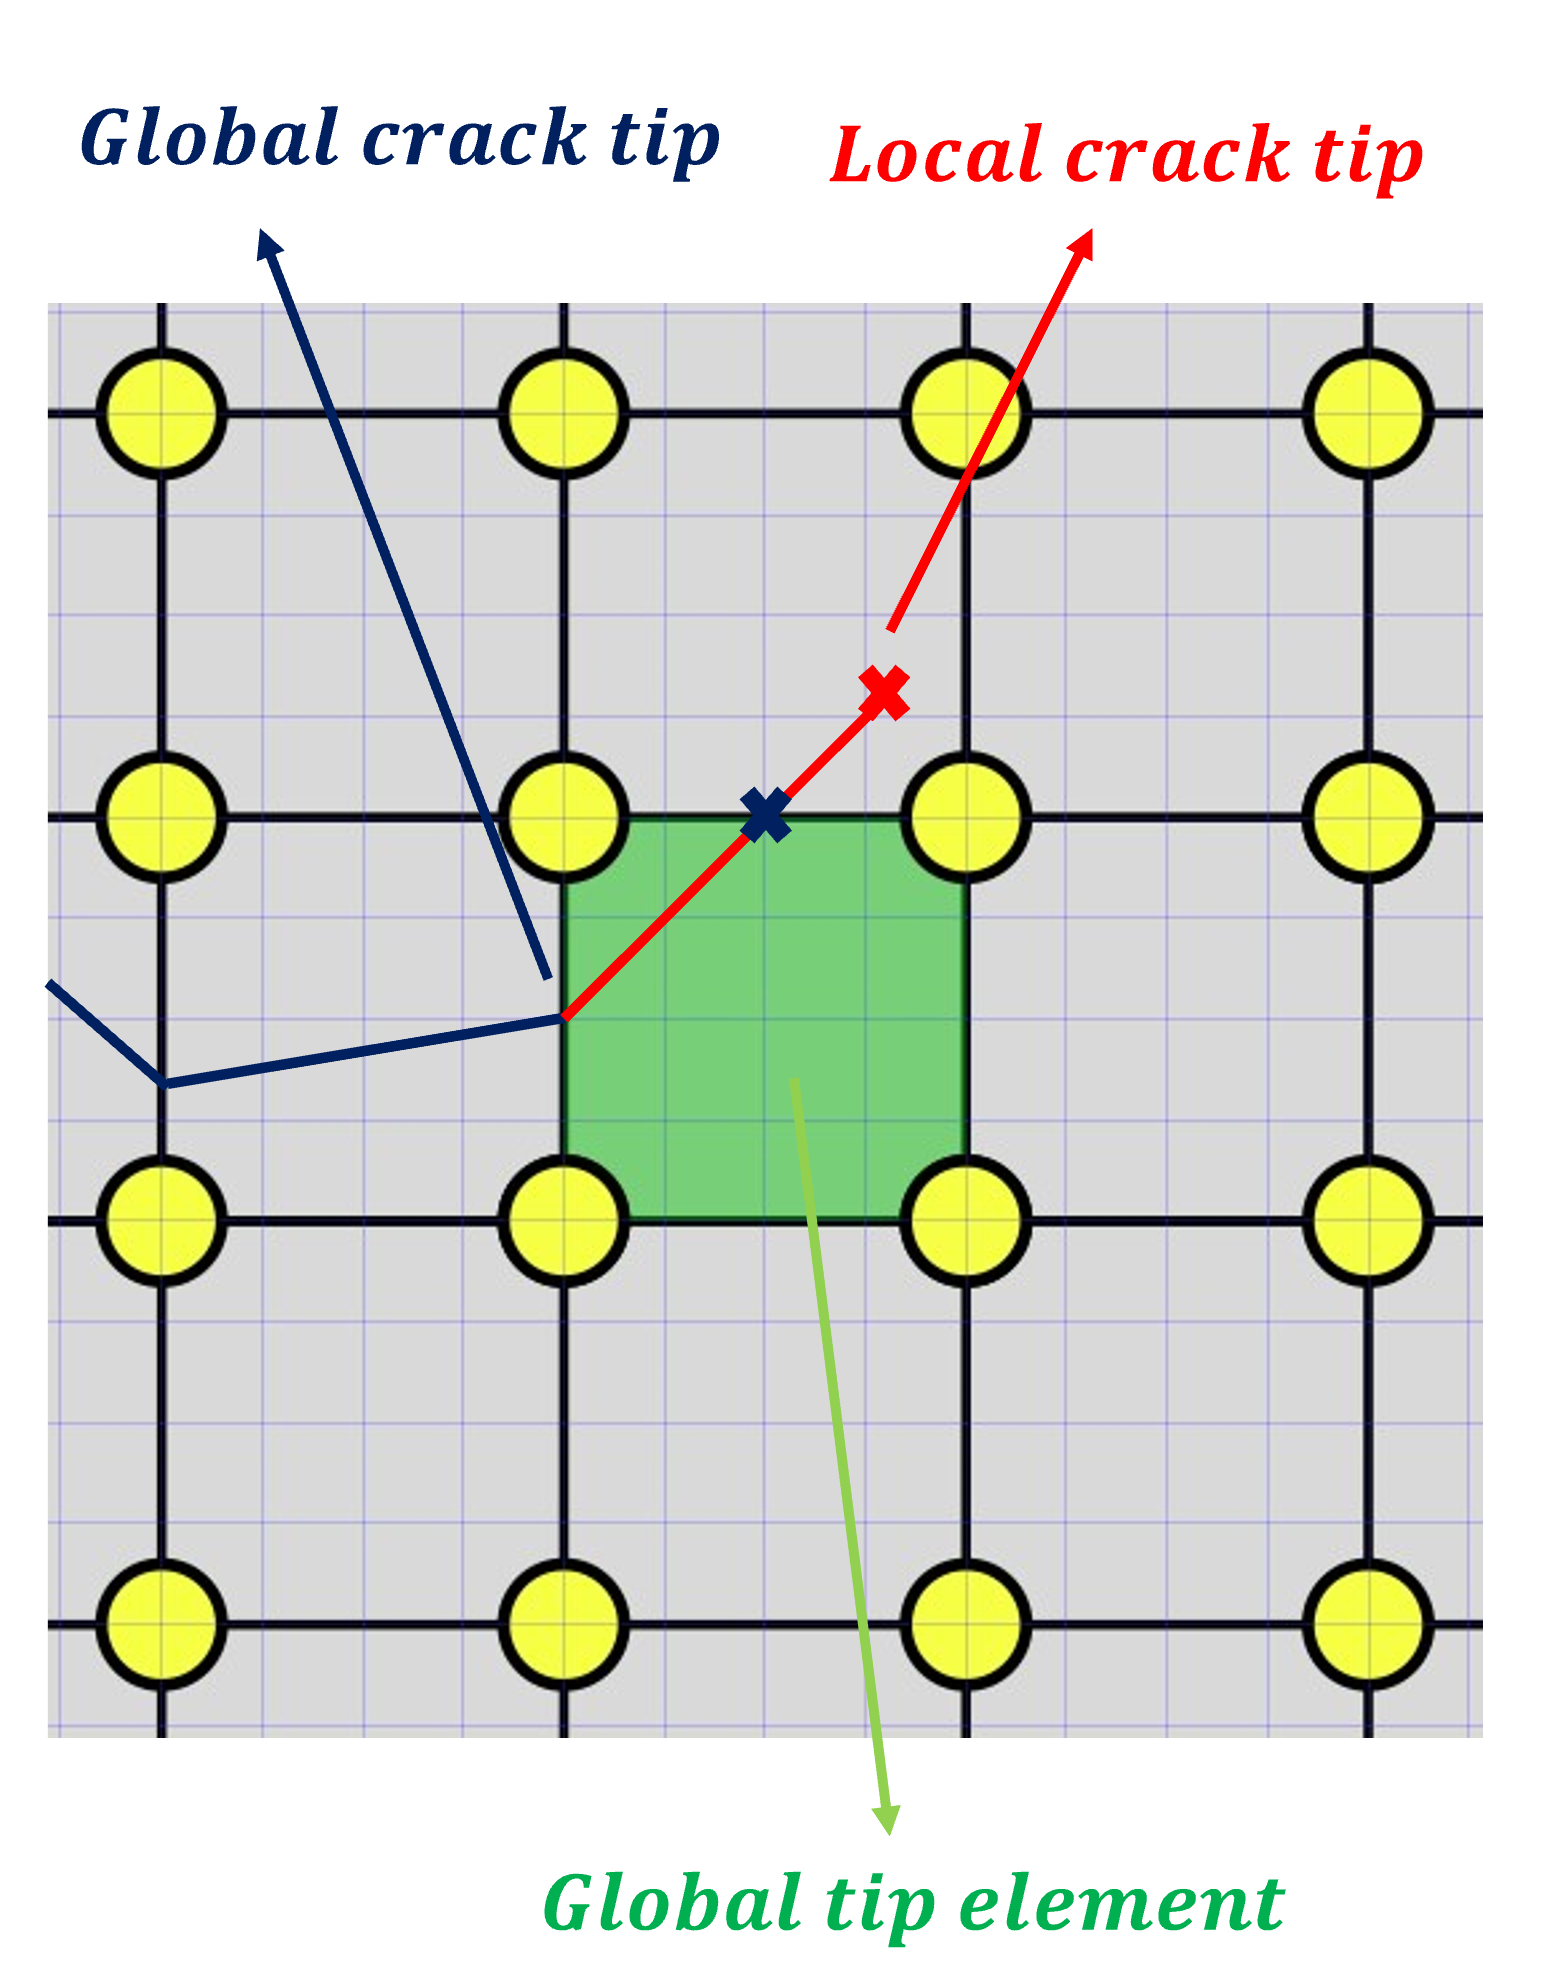
\includegraphics[width=.99\linewidth]{img/Section2/schematic_1.png}
  \caption{}
  \label{fig:prop_1}
\end{subfigure}%
\begin{subfigure}{.33\textwidth}
  \centering
  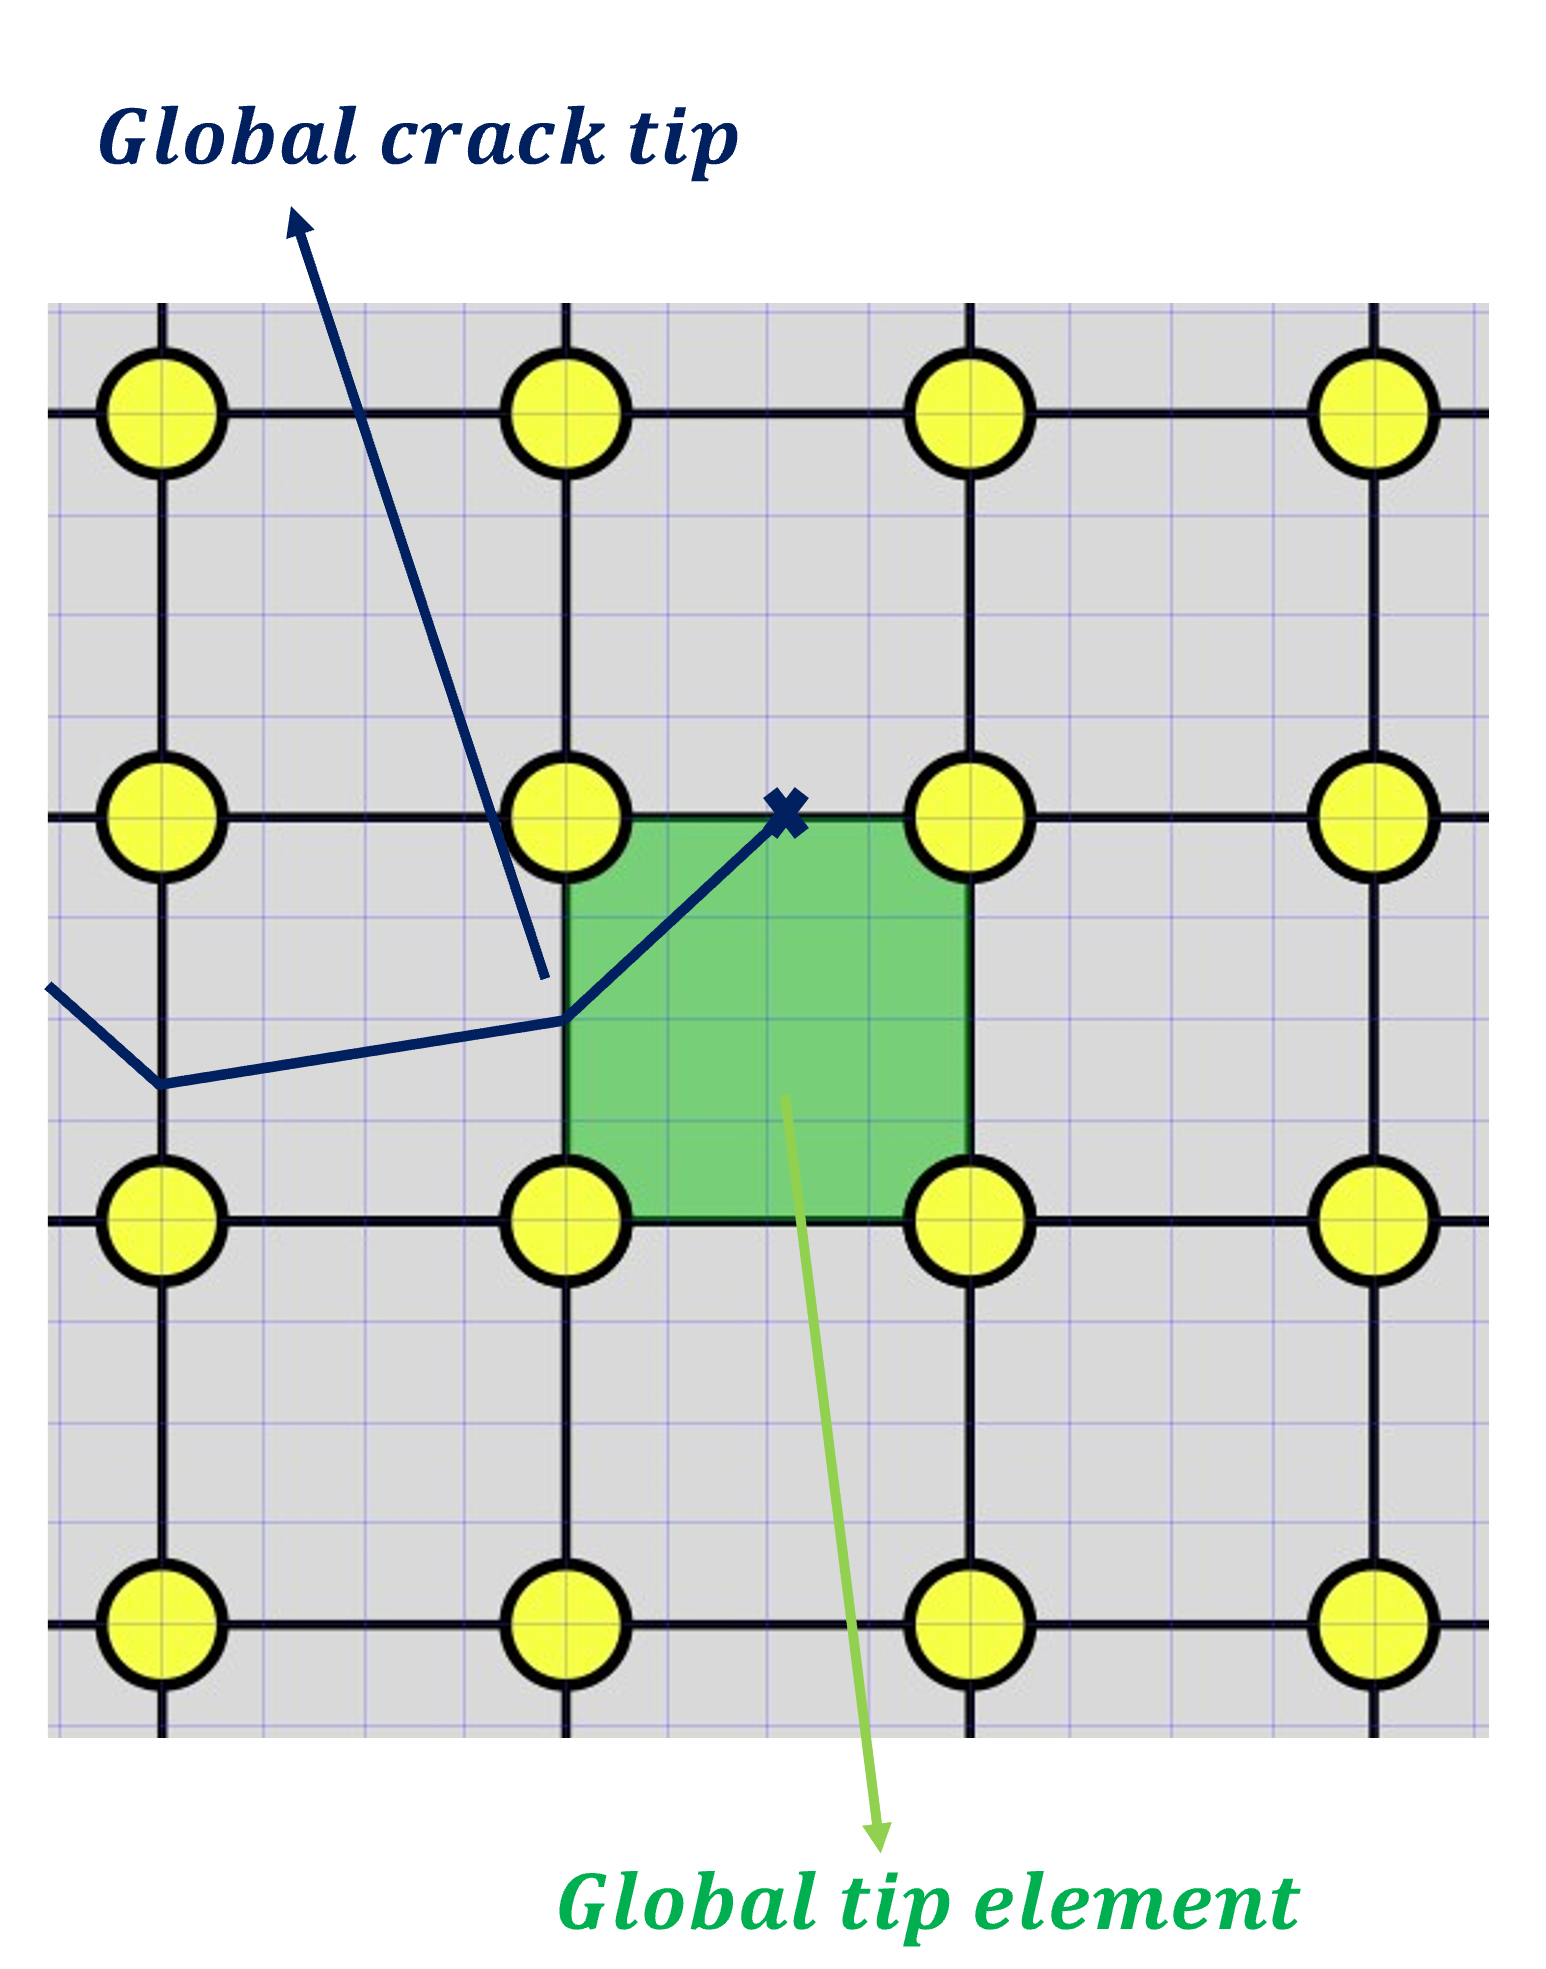
\includegraphics[width=\linewidth]{img/Section2/schematic_2.png}
  \caption{}
  \label{fig:prop_2}
\end{subfigure}
\begin{subfigure}{.33\textwidth}
  \centering
  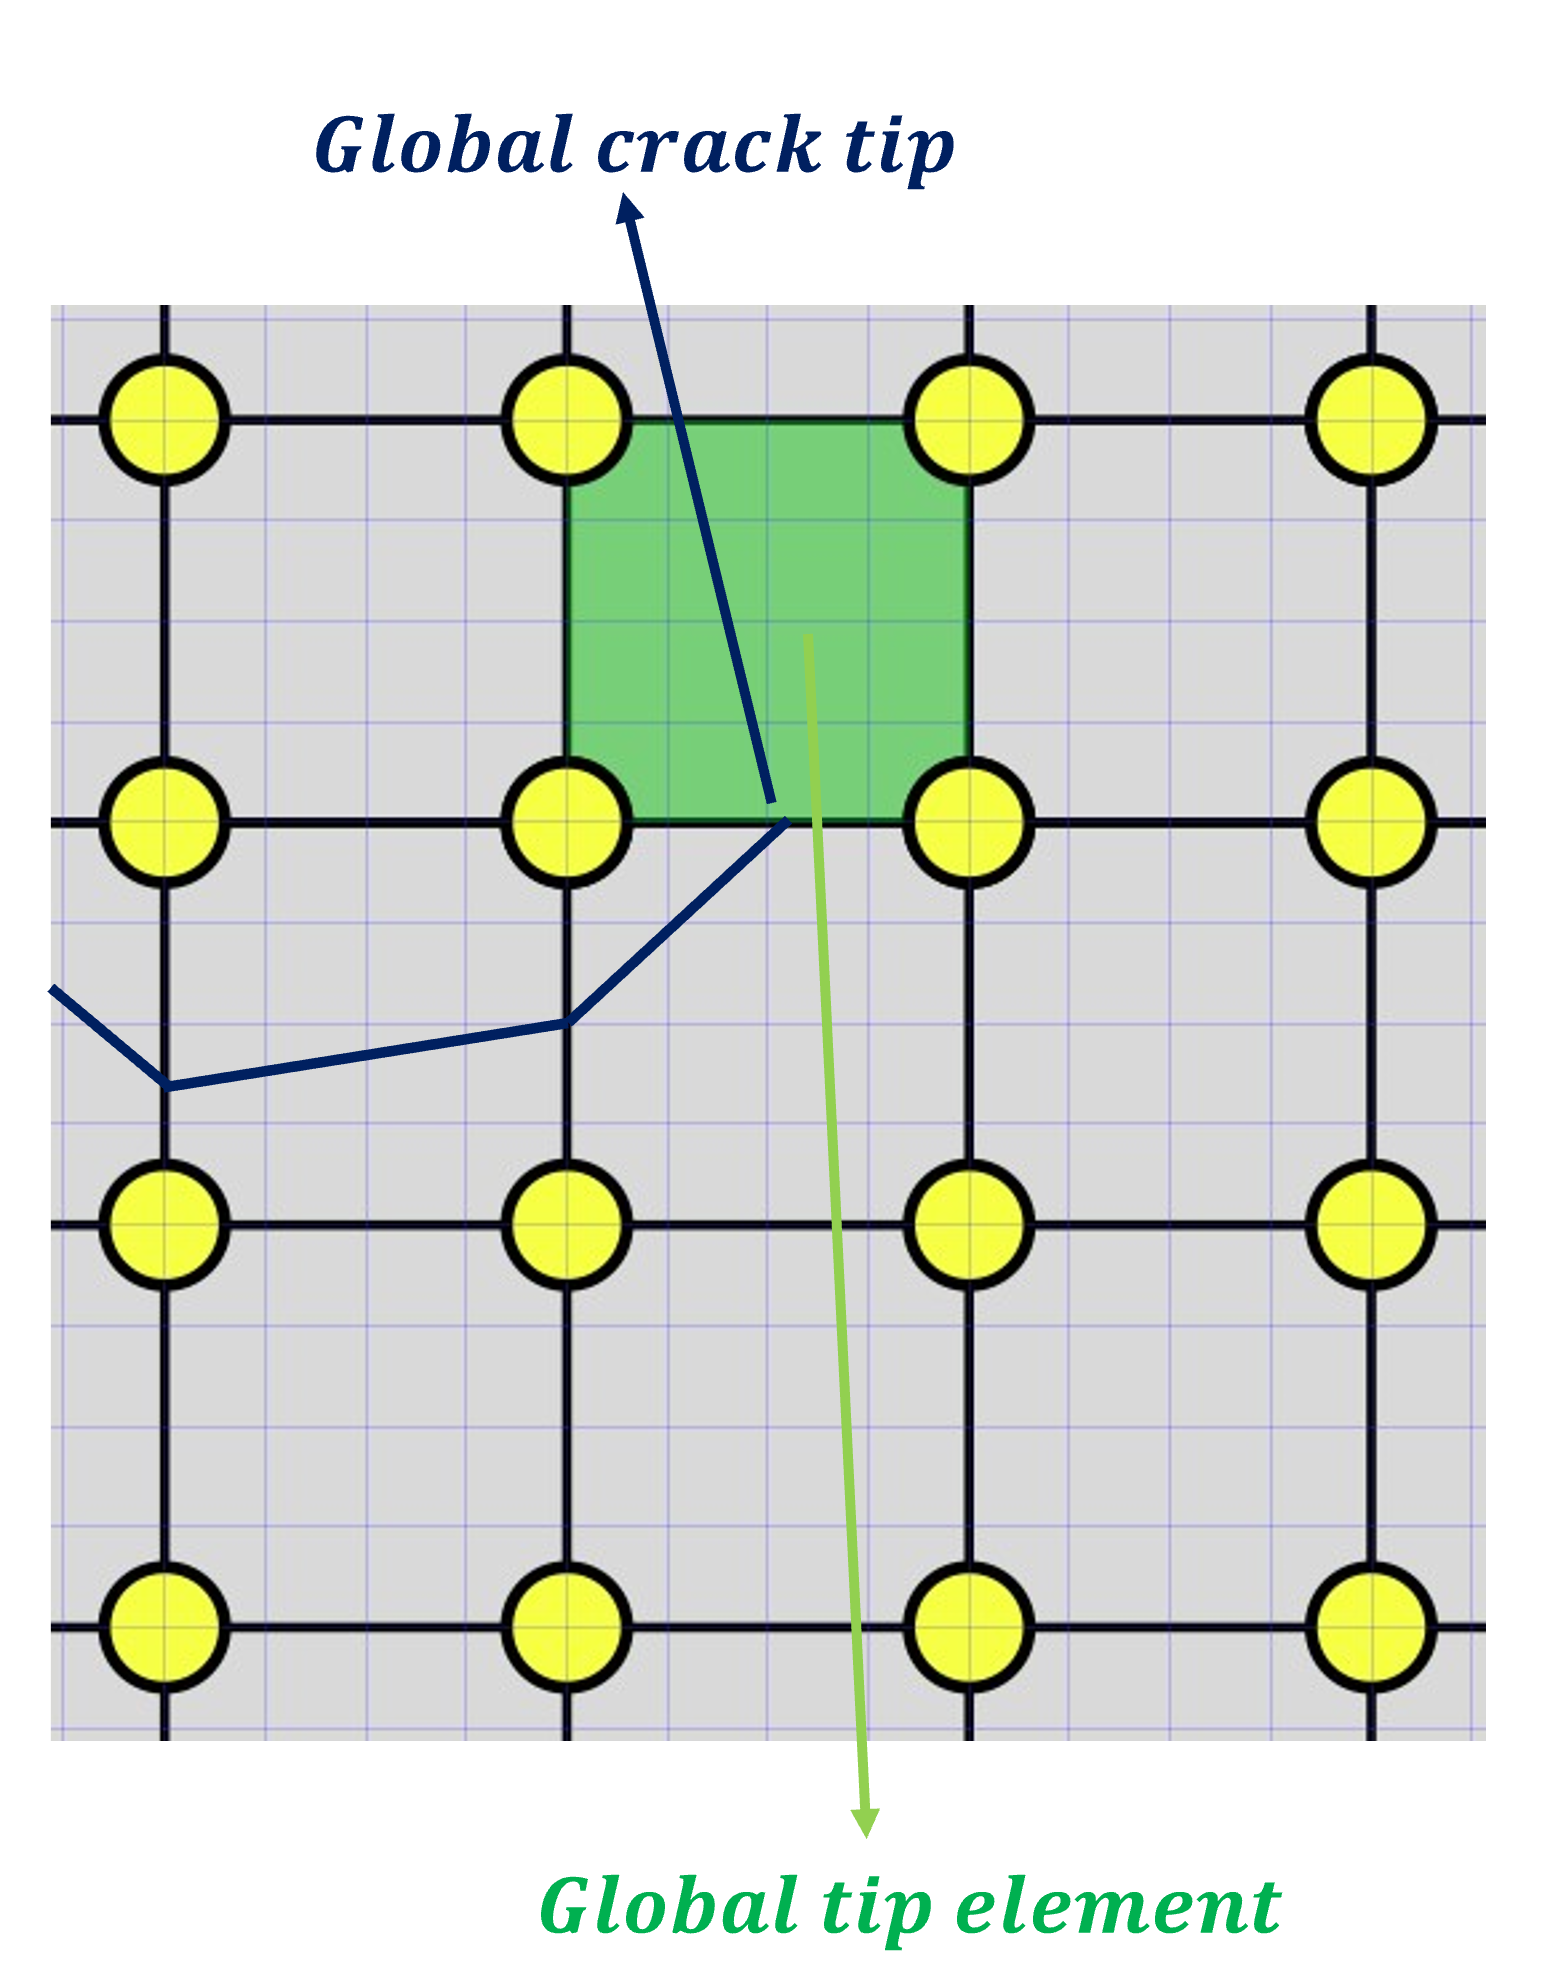
\includegraphics[width=\linewidth]{img/Section2/schematic_3.png}
  \caption{}
  \label{fig:prop_3}
\end{subfigure}
\caption{(a): Construction of the segment connecting global and local tips.  (b) New crack segment to be added. (c) Update of the global crack tip and global tip element.}
  \label{fig:tip_progression}
\end{figure}

In general, the problem of extracting a sharp crack front from a diffuse representation is not trivial. When the crack evolution involves complex topological changes, it is particularly difficult\cite{tamayo2015medial}. In the numerical examples studied in this manuscript, we take advantage of the relatively simple fracture geometry and predicted crack patterns to simplify this process.  In particular, we first identify all elements in the local subdomain with nodes whose damage values are all above a threshold $d_{tr}$. A similar approach was proposed in \cite{giovanardi2017hybrid}. The local crack tip is taken to be the center of the element in this set that is farthest from the base of the crack in the local subdomain.  The threshold used for this process is taken to be $d_{tr} = 1 - h_{local}/(2\ell)$, which is based on the estimate for a damage field near a crack tip given in \cite{yoshioka2020crack}. In essence, for a phase-field model of fracture, this threshold identifies nodes that are expected to correspond to the peaks of the discrete damage field.  For a damage band resolved with a mesh spacing of $\ell / h_{local} = 4$, this gives rise to a threshold of  $d_{tr} = 0.875$. 

\subsection{Algorithm summary}

Having described the solution strategies for both the global and local problems and the transfer of various quantities, we now detail the algorithm \eqref{mr_algorithm} that couples the two problems together to simulate crack propagation. Figure~\ref{fig:solution_algorithm} provides an illustration of the algorithm. Within each time step (outer loop), the algorithm employs an inner loop that allows the global problem to be updated as soon as any large enough change in the crack geometry is detected in the local subproblem.  The inner loop is terminated when the propagation step, described in subsection \ref{propagation_step} does not identify any crack advance.  The construction with two nested loops can be viewed as an implicit treatment of the fracture front position, which, according to Lecampion et al.\ \cite{lecampion2018numerical} tends to be more accurate and robust, permitting the use of larger time steps.

\medskip

\begin{algorithm}[H]\label{mr_algorithm}
\small
\SetAlgoLined
 Define initial and boundary conditions
 
 $n = 1$ \\
 $n_F = endStep$
 
 \While{$n \le n_F$}{
 
    \medskip
    
    $\mathcal{F}_n^{1} = \mathcal{F}_{n-1}$
 
    \For{$1 \le k \le maxIter\footnote{The index $k$ is only a dummy variable for this loop that searches for the correct fracture geometry at a given time step.}$}{

    \medskip
    
    (1) Solve \textbf{Global Problem} and obtain $\textbf{u}_G^{k,n}, p_m^{k,n}, p_f^{k,n}$

    \medskip
    
    (2) Construct subdomain $\Omega_L$ and submesh $\mathcal{T}_L$. Identify subset of cracked nodes $\mathcal{K}$.
    
    \medskip
    
    (3) Prescribe local boundary conditions $\textbf{u}^h_{L}|_{\partial\Omega_L} = \textbf{u}_G^{k,n}|_{\partial\Omega_L}$ and $d^h = 1$ on $\mathcal{K}$.
    
    \medskip
    
    (4) Construct local pressure fields $p_m= \Pi^{\Omega_L}_m (p_m^{k,n})$ and $p_f = \Pi^{\Omega_L}_f (p_f^{k,n})$
    
    \medskip

    (5) Solve the \textbf{Local Problem} to obtain $d^{k}$.

    \medskip
    
    (6) Use $d^{k}$ and the propagation step (subsection \ref{propagation_step}) to update discrete fracture $\mathcal{F}_n^{k}$.

    \medskip
    
    \If {$\mathcal{F}_n^{k+1}$ = $\mathcal{F}_n^{k}$}{
    
        \medskip
    
        n = n + 1
        
        \medskip
        
        $\mathcal{F}_n = \mathcal{F}_n^{k}$
        
        \medskip
            
        $\textbf{u}_G^n = \textbf{u}_G^{k,n}$
        
        \medskip
            
        $p_m^n = p_m^{k,n}$
        
        \medskip
        
        $p_f^n = p_f^{k,n}$
        
        \medskip
            
        break
        
        \medskip
    
        }

    }
    
 }
 \caption{Solution algorithm for multi-resolution hydraulic fracture}
\end{algorithm}

\begin{figure}[h]
    \centering
    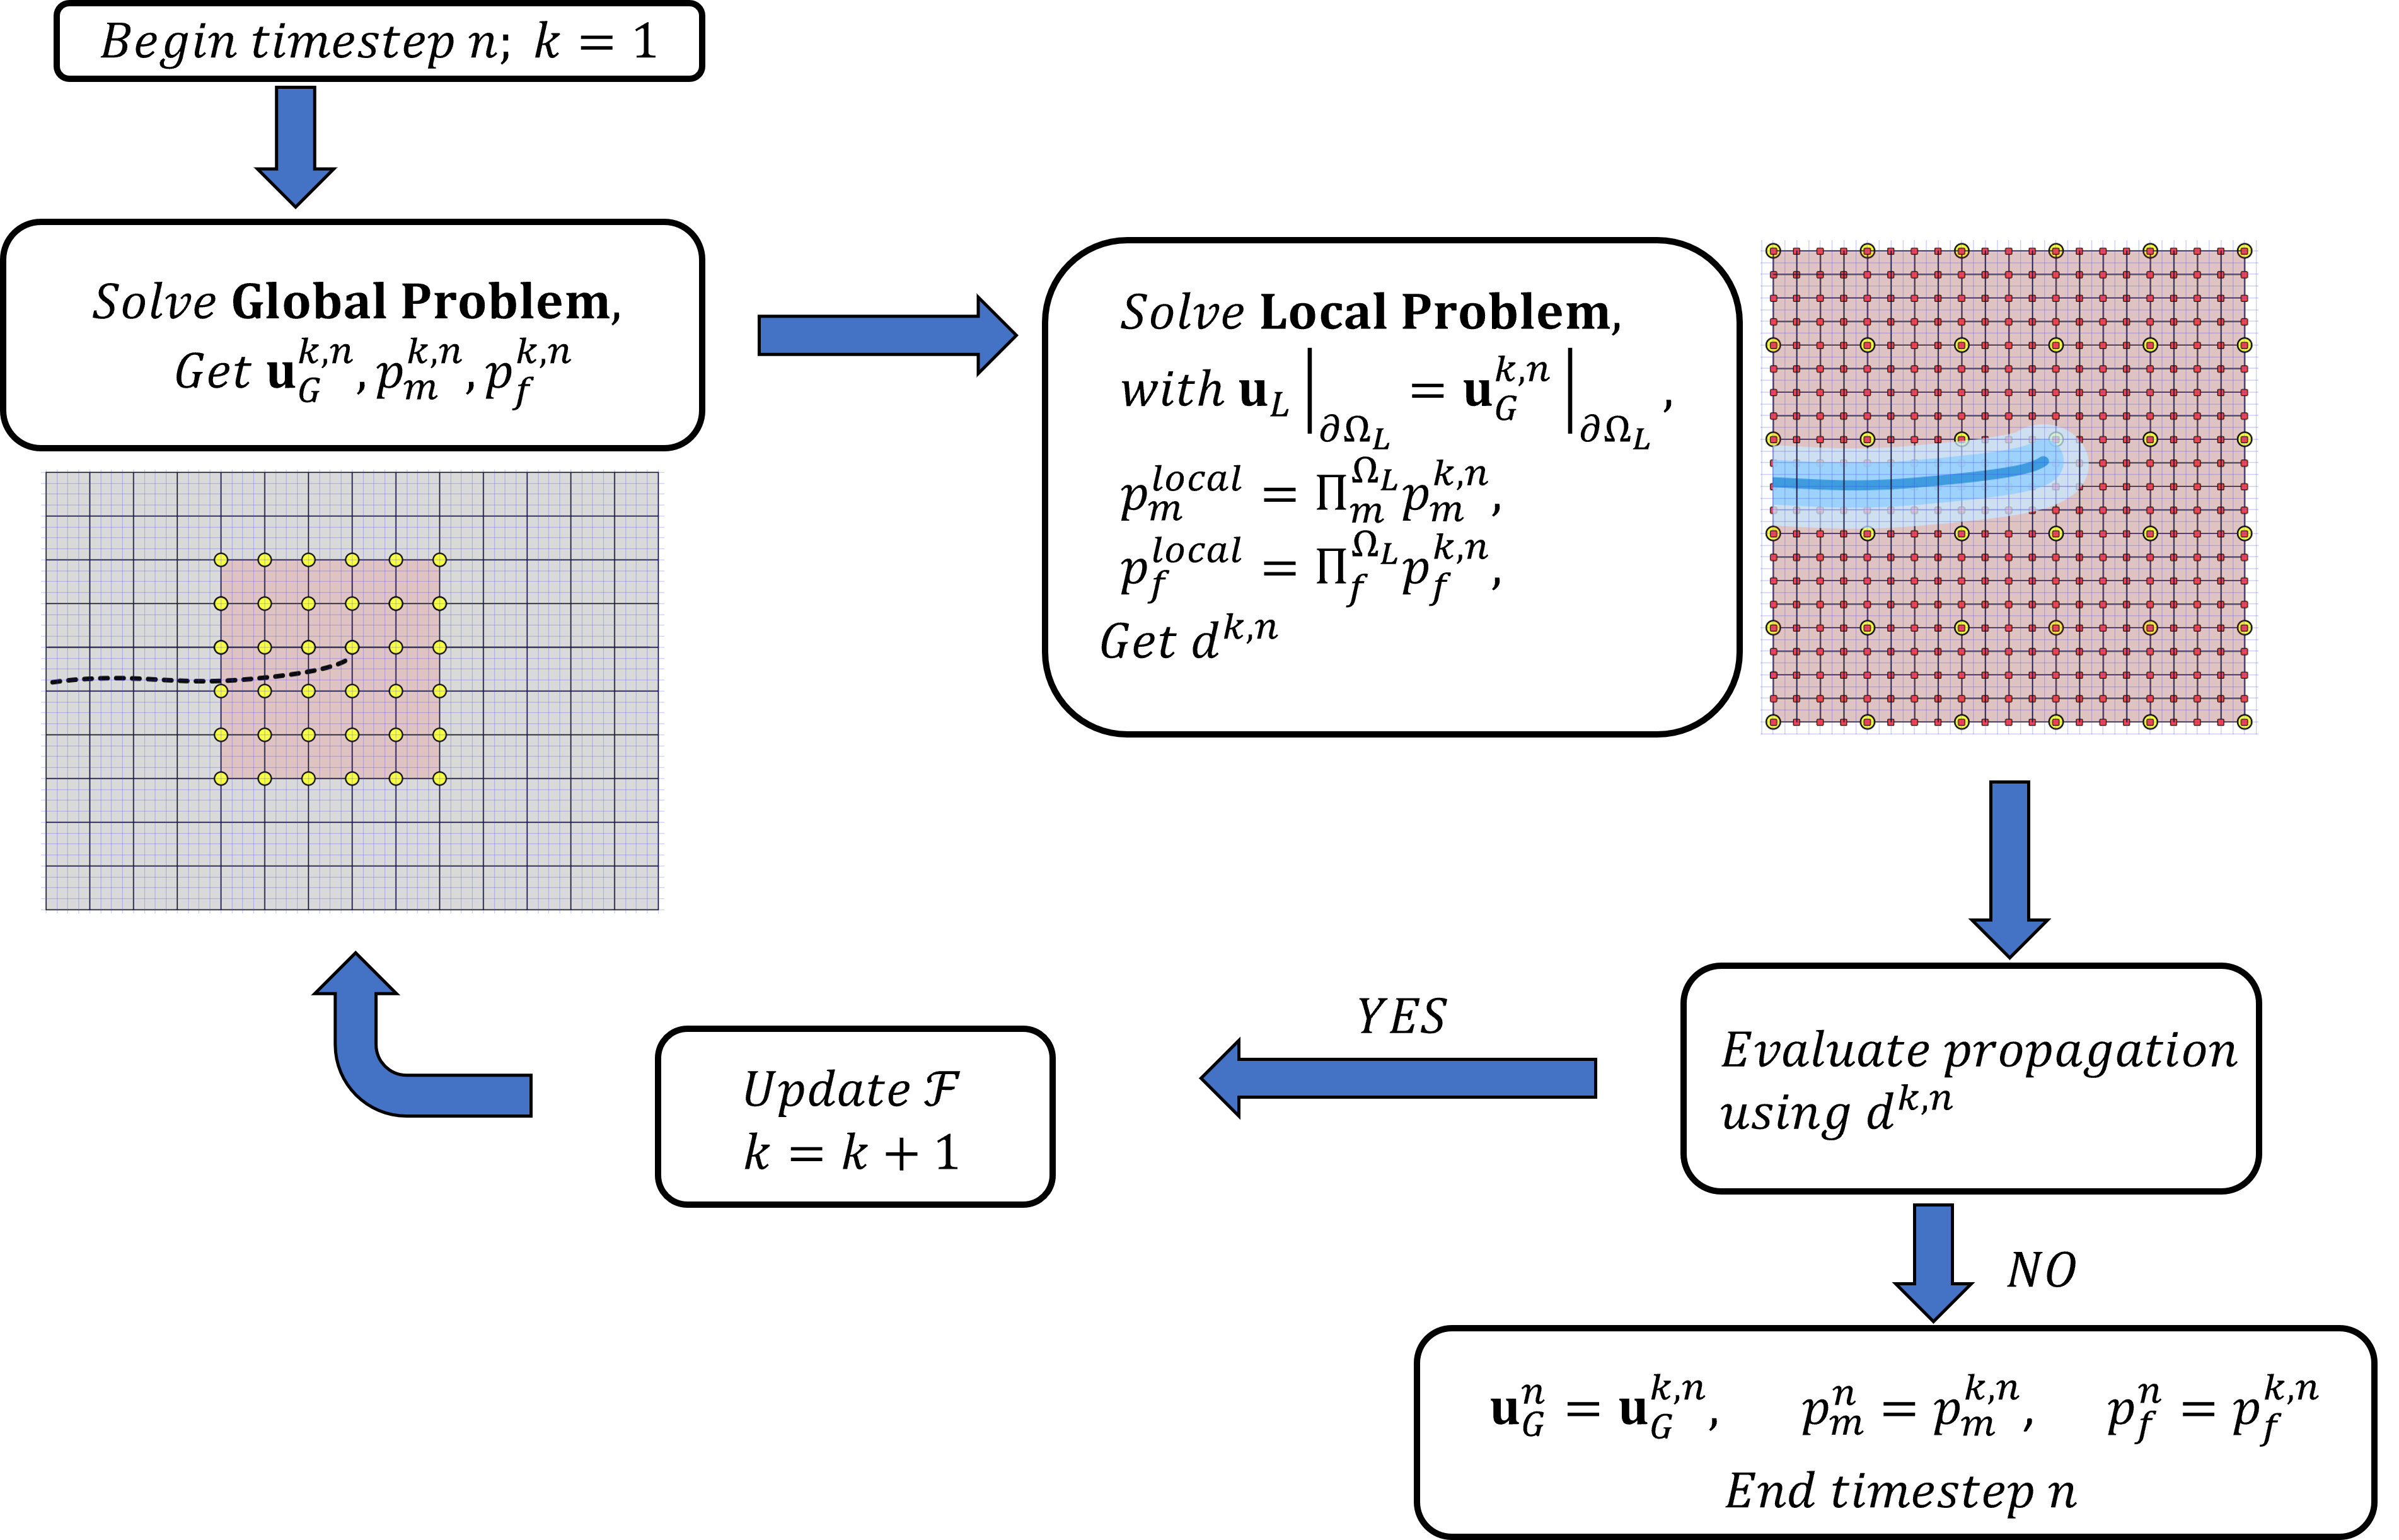
\includegraphics[width=\linewidth]{img/Section2/algorithm_fancy.png}
    \caption{Multi-resolution solution algorithm.}
    \label{fig:solution_algorithm}
\end{figure}
